\documentclass{article}

\usepackage[utf8]{inputenc}
\usepackage[left=1.5in,right=1.5in,bottom=1in]{geometry}
\setlength\parindent{0pt}
\setlength{\parskip}{1em}
\setcounter{secnumdepth}{0}
\usepackage{outlines}
\usepackage{graphicx}
\graphicspath{ {imgs} }
\usepackage{hyperref}
\usepackage{color,soul}

\newcommand{\alignedmarginpar}[1]{%
        \marginpar{\raggedright\small #1}
    }

\title{Urban Social Geography - Summarised Notes}
\author{Carla Hyenne }

\begin{document}

\maketitle

\tableofcontents

\pagebreak

\pagebreak\section{Urban Geographical Traditions}

\textbf{Globalised urbanisation}: urbanisation is a global phenomenon. It is also unequal across the world (eg. Asia dominates economic growth and urbanisation). The `urban age' frame can be criticised:\alignedmarginpar{Brenner and Schmid, 2014} measurements depend on diverging national definitions, and it is a chaotic abstraction that does not neatly overlay cities in a spatial sense.\alignedmarginpar{Urban vs. Rural}

\textbf{The urban}: a distinctive way of life, which can take place in the city but also outside (suburbs, rural, slums). It epitomises a particular society (capitalist, industrial, fordist, modern, classist, etc.). It projects symbolic power, notably by means of its built environment.

\textbf{The city}: the material built environment. Has a complex division of labour, with increasing efficiency and surplus, but also inequalities. It projects symbolic power\alignedmarginpar{Skyscrapers (Dubai, NYC); CCTV tower (Beijing)}, and has physical and administrative boundaries. The `non-city' is hard to define, because it's hard to know where the city ends: the `rural', the peripheries, can have elements of the city.

\textbf{Urbanisation}: the process of becoming urban. It is a demographic process, whereby cities gain more and varied residents, with increasing density. It entails a globalisation of urban economic, political and cultural influence. It considers how space is organised through processes of uneven development.

\textbf{Geography}: the social and physical processes within the context of space. There are multiple concepts of space: \textbf{territory}, the boundaries and sovereignty of a space\alignedmarginpar{Brussels capital}; \textbf{scale}, the sensitivity of processes; \textbf{network}, hubs and leaks beyond the territory, towards micro-networks; and \textbf{place}, the attachement of meaning and sentiment to a space.

\textbf{Critical geography}:\alignedmarginpar{Jonas et al., Sayer, Brenner and Schmid} epistemological rules of thumb include: acknowledging that there is no universal theory of anything; knowing every theory has birthmarks, ie. is situated in time and space, and reflecting on the birthmarks is necessary to be critical\alignedmarginpar{provincialisation}; asking whether theories can be used across contexts; engaging in pluralism to allow inter-theoretical conversation and comparison.

\textbf{Materialist approaches to geography}: concerned with the distribution and social-justice, and agenda-setting.

\textbf{Humanist approaches to geography}: about the experienced city, issues of representation and discourse, uses qualitative methods, gives a voice.

\begin{center}
	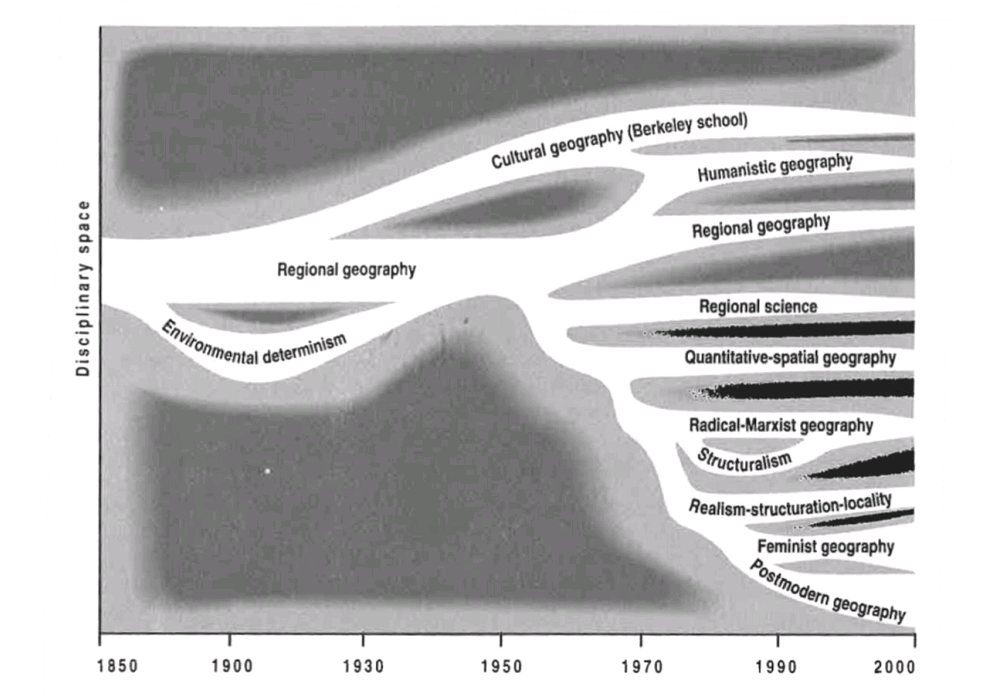
\includegraphics[width=23em]{geography_approaches.png}
\end{center}

\pagebreak\section{Theories of World-City Formation}

\textbf{Measuring centrality of cities/city-regions}:\alignedmarginpar{Deltametropolis, Flemish Diamond, RheinRuhr, Ile-de-France, Greater London}there are multiple ways to measure the power of cities or regions, like the weight of the area in the national context (regarding GRP, density...), the number of patents, the level of education, the proportion of employment per sector (higher in the service sector than industry or agriculture).

\textbf{World cities}:\alignedmarginpar{Friedmann}world cities are points of functional centrality, serving command and control functions in a global urban system, where processes cross national borders. The world economy is restructured, there is a new international division of labour (offshoring), TNCs and MNCs dominate the global supply chain that is highly integrated.
This creates uneven socio, economic and spatial developments because of a hierarchy connecting the core (absorbing the surplus) and the periphery.

\textbf{Global cities}:\alignedmarginpar{Sassen}path dependencies concentrate Advanced Producer Services in select cities. The path dependencies include the extensive services market providing access for firm/client relations, the labour market and associated culture, the APS complex and the cross-border connections offered by its network. 
APS have control capabilities and \textbf{polarise the labour market} (high and low-skilled labour required). This results in the \textbf{peripheralisation} of the core.

\textbf{Global city regions}:\alignedmarginpar{Scott\\Silicon Valley, Pearl River Delta}a complex assemble of cities, settlements, hinterlands that are interconnected by production networks, themselves oriented towards the global economy. An urban core is not always required for a region to be central in the post-Fordist industry (ie. service and knowledge industries). APS can still be an indicator for global city regions.

\textbf{GaWC heuristic}: used to map the world-city network. Assumption is that the presence of international APS firms can be used to indicate the presence of command-and-control functions of cities.

\textbf{Post-colonial critique}:\alignedmarginpar{Robinson} the western bias in urban knowledge production leaves places off the map of urban studies. Off the geographical map (global South), and off the conceptual map (limited economic processes, ignores inter-urban connections). World cities research ignores `ordinary' cities in the global economy.

\textbf{Social-constructivist critique}:\alignedmarginpar{Massey}the world-cities are politically constructed, and their consequences are un-debated and hide other realities\alignedmarginpar{London's financial centre vs. low-skilled labour}. World cities are not a given but a product of local and global forces, mediated by acts of representation (financial and political elites, or policies that promote the city).

\textbf{Political-economy critique}:\alignedmarginpar{Brenner}there is a rescaling of the state due to globalisation, which changes the political and economic scales to supra and sub-national levels. There are new governance structures, a shift from managerialism to entrepreneurialism\alignedmarginpar{inter-urban competition}, global accumulation regimes are centred on (global) cities, their importance reinforced by global city building agendas.

\textbf{Financialisation critique}:\alignedmarginpar{Bassens \& van Meeteren}the deregulation of financial markets has financialised firms who are mostly present in APS complexes. Unfortunately this leads to global financial crises, and tax evasions.

\pagebreak\section{Polarisation in World/Global Cities}

\textbf{Polarisation}:\alignedmarginpar{Friedmann and Wolf, citadel vs. ghetto}a class division that is reproduced through space, and is stronger in global cities. Polarisation is explained by an \textbf{economic restructuring}\alignedmarginpar{North-Atlantic}. Productivity has increased, but wages have not because profit is invested elsewhere (eg. financialisation)

\textbf{Economic restructuring}: post-Fordism restructured the economy. Production was relocated (globalisation, NIDL); deindustrialisation declined activity in the city; structural unemployment; shift towards fiscal austerity\alignedmarginpar{declining tax base}; market rationality and privatisation\alignedmarginpar{neoliberalism}; shift from state to market control over multinational capital; inter-urban competition.

\textbf{Harvey's entrepreneurial strategies}: \textbf{Production}: policy makers create/exploit certain advantages for the production of goods and services; forms clusters and edge cities. \textbf{Consumption}: improving the city's position in the spatial division of consumption; affects socio-spatial structure. \textbf{Redistribution}: competition for (supra)nationally redistributed surplus from the economy. \textbf{Command and control}: investing in high finance, government, and information economy; forms monopoly spaces in global/world cities.

\textbf{Polarisation thesis}:\alignedmarginpar{Friedmann \& Wolff; Sassen}the change in economic base led to a decline of well-paid manufacturing job (exodus) and a growth in service jobs (formal \& informal) with an influx of high-salaried workers (professional and managerial jobs) and low-skilled workers to support their lifestyle and routine service jobs. Creates an ``hourglass'' of ``upper circuit''/``underclass''.\alignedmarginpar{urban elite networks}

\textbf{Labour market globalisation}: global cities have high-paid and low-paid migrants, often divided ethnically.\alignedmarginpar{expat vs. immigrant} Growing supply of low-skilled migrant labour for typically 3D jobs (dirty, demanding/difficult, dangerous) drives wages down. There is growing informality and a \textbf{``peripheralisation at the core''}\alignedmarginpar{Sassen-Koob}, where exploitation not only takes place in the global South but also global North where the `peripheralised' live. \textbf{New forms of industrial exploitation} in \alignedmarginpar{sweatshops}global cities are made possible by the absence of regulation in the (global) periphery.

\textbf{Criticism of polarisation in global cities}: universalising and generalising tendencies, but does the logic apply elsewhere than NY-LON-TOK? Simplistic theory that reduces complexity of occupational and spatial structures, and professionalisation and mobility can also impact socio-spatial inequalities.

\textbf{Occupational structure}:\alignedmarginpar{Hamnett}professionalisation means high-income jobs are growing, and doesn't necessarily mean growth of low-paid jobs. There is an `upgrading' of the labour market, and better welfare states\alignedmarginpar{minimum wage} prevent extreme polarisation. Labour inequalities emerge because of market exclusion based on gender and ethnicity.

\textbf{Spatial structure}: statistics could exaggerate polarisation. Suburbanisation of the middle class could mean that middle-incomes are not disappearing but moving outside of the city. High-end housing demand drives super-gentrification\alignedmarginpar{Lees, 2003\\Brussels, Brooklyn}. Influence of pre-existing spatial forms and path dependencies. 

\textbf{Three-layer model}:\alignedmarginpar{Burgers and Musterd, 2000}for analysing inequality in cities: macro-level (global change, economic restructuring, increasing mobility of capital, people, commodities, information); micro-level (individual level, change in labour opportunities in a specific local context); medium-level (connects global and local, national institution differences, different urban trajectories)\alignedmarginpar{Charleroi/Detroit}

\textbf{Future}: income polarisation is expected to expand due to austerity, the flexibilisation of the labour market, migration labour, and political wealth.

\pagebreak\section{Urban Segregation: Patterns and Causes}

\textbf{}

\textbf{}

\textbf{}

\textbf{}

\textbf{}

\textbf{}

\textbf{}

\textbf{}

\textbf{}

\pagebreak\section{Neighbourhood Effects and Living with Diversity}

\textbf{}

\textbf{}

\textbf{}

\textbf{}

\textbf{}

\textbf{}

\textbf{}

\textbf{}

\textbf{}

\pagebreak\section{Cultures of Urban Research}

\textbf{}

\textbf{}

\textbf{}

\textbf{}

\textbf{}

\textbf{}

\textbf{}

\textbf{}

\textbf{}

\pagebreak\section{Urban Cultures}

\textbf{}

\textbf{}

\textbf{}

\textbf{}

\textbf{}

\textbf{}

\textbf{}

\textbf{}

\textbf{}

\pagebreak\section{Transport and Cities: a Historical Hegemony}

\textbf{}

\textbf{}

\textbf{}

\textbf{}

\textbf{}

\textbf{}

\textbf{}

\textbf{}

\textbf{}

\pagebreak\section{Critical Perspective on Urban Transport}

\textbf{}

\textbf{}

\textbf{}

\textbf{}

\textbf{}

\textbf{}

\textbf{}

\textbf{}

\textbf{}

\end{document}
